\section{Step 1: Encrypted Machine Learning}
\begin{frame}{\gls{ppml}}
  \begin{itemize}
    \item Machine Learning allows us to solve otherwise difficult problems.
    \item Development of new applications and solutions 'of numerical nature' in different fields
          \begin{itemize}
            \item Example: Health Care with highly sensitive medical data.
            \item Even more volatile results: disease indicators.
          \end{itemize}
    \item $\Rightarrow$ Demand for privacy-preserving solutions in \gls{ml} applications.
  \end{itemize}
\end{frame}

\begin{frame}{Feedforward Neural Networks}
  \begin{figure}[H]
    \centering
    \scalebox{0.9}{\inputtikz{figures/neural-network}}
    \caption[Neural Network illustration resembling the one used in our demonstrator]{
      The simple neural network used in our demonstrator with $\vec{h} = \cryptop{relu}(M_1 \vec{x} + \vec{b_1})$ and the output $\vec{y} = \cryptop{softmax}(M_2 \vec{h} + \vec{b_2})$.
    }
    \label{fig:neural-network}
  \end{figure}
  \vspace{6pt}
  $\Rightarrow$ Need: Addition, Multiplication, Packing, Rotations. Trained in plain.
\end{frame}

\begin{frame}{Goal: Classify MNIST Images of Handwritten Digits}
  \begin{itemize}
    \item Two major types of \gls{ml}: Supervised and Unsupervised Learning
    \item Popular dataset: \gls{mnist}. Encode as vector of 784 entries.
  \end{itemize}

  \begin{figure}[H]
    \centering
    \scalebox{0.8}{\inputtikz{figures/mnist}}
    \caption[Sample images of the MNIST dataset]{
      Sample images of the MNIST database of handwritten digits \parencite{mnist-original}.
      The dataset contains 70,000 images of $28 \times 28$ greyscale pixels valued from 0 to 255 as well as associated labels (as required for supervised learning).
    }
    \label{fig:mnist}
  \end{figure}
\end{frame}

\begin{frame}{Secure Handwritten Digit Classification as a Service - Demo}
  \begin{columns}[c]
    \begin{column}{0.7\linewidth}
      \begin{figure}[H]
        \centering
        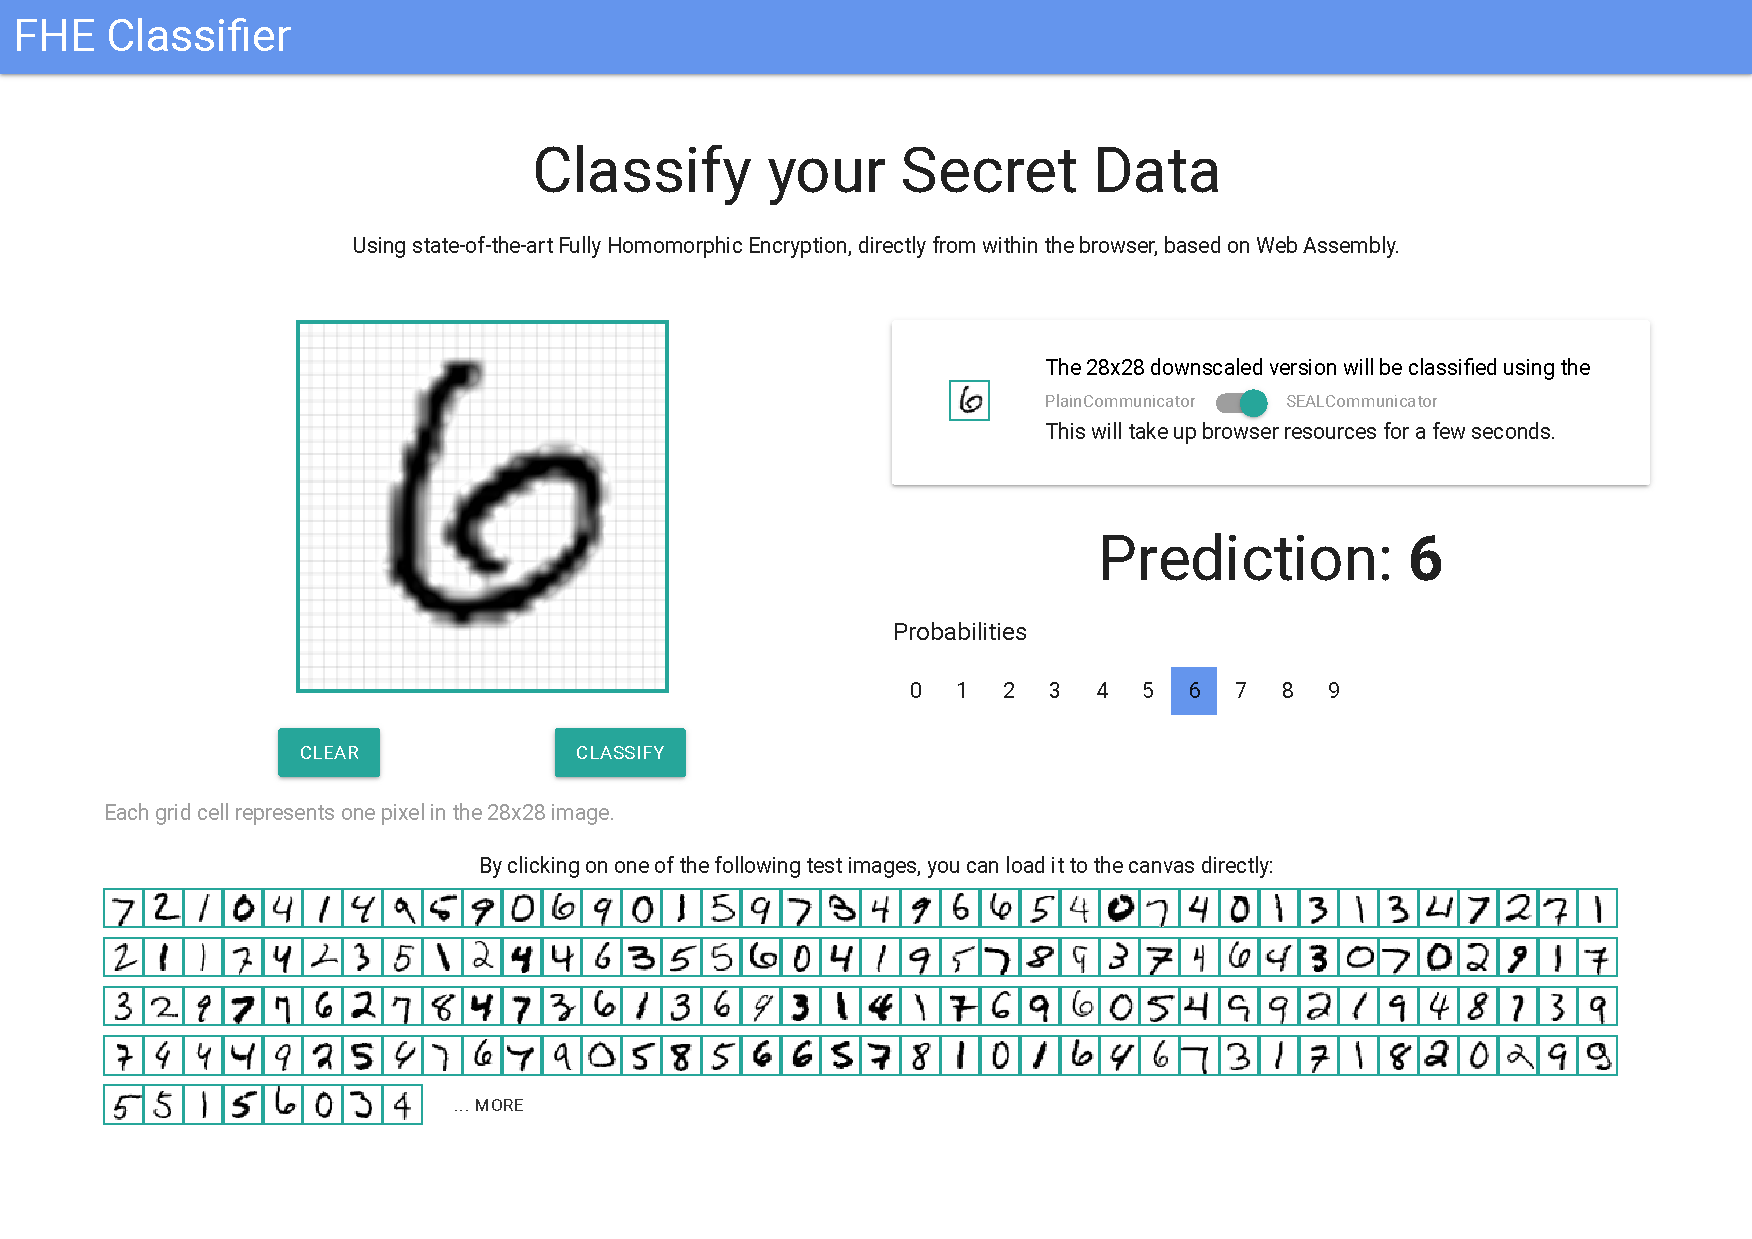
\includegraphics[width=0.75\linewidth]{../thesis/figures/frontend.pdf}
        \vspace{-0.3cm}
        \caption{\url{https://secure-classification.peter.waldert.at/}.}
      \end{figure}
    \end{column}
    \begin{column}{0.24\linewidth}
      Scan the QR-Code:
      \qrcode[nolink,height=3.1cm]{https://secure-classification.peter.waldert.at/}
    \end{column}
  \end{columns}
\end{frame}
